% KansasLava-AK.tex
\begin{hcarentry}{Haskell Equational Reasoning Model-to-Implementation Tunnel}
\label{HERMIT}
\report{Andy Gill}%11/10
\participants{Andrew Farmer, Ed~Komp, PostDoc (TBA)}
\status{ongoing}
\makeheader

The Haskell Equational Reasoning Model-to-Implementation Tunnel (HERMIT) is an NSF-funded project being
run at KU to improving the Applicability of Haskell-Hosted Semi-Formal Models to High Assurance Development.

In engineering practice, models are an essential part of understanding how to build complex systems. In this project, high-level models and efficient implementations of computer systems will be developed side-by-side under a single framework that bridges the gap between them using a high degree of automation. This is possible due to the use of a modern functional language for both the model and implementation, and the deployment of a new and powerful general-purpose and semi-automatic refinement technology.

The functional language Haskell has already enjoyed considerable success as a platform for high-level modeling of complex systems with its mathematical-style syntax, state-of-the-art type system, and powerful abstraction mechanisms. In this project, Haskell will be used to express a semi-formal model and an efficient implementation, taking the form of two distinct expressions of computation with the same mathematical foundation. The project develops tools and methodologies that use transformations like the worker/wrapper transformation to construct links between these models and implementations, lowering the cost of the development of high-assurance software and hardware components in application areas like security kernels and critical control systems. Lowering the cost of linking semi-formal specifications and models to real implementations will have considerable impact. For example, Evaluation Assurance Level (EAL) 5 and 6 of the Common Criteria call for semi-formal methods to construct such link, and this project addresses keys part of this requirement. 

\begin{center}
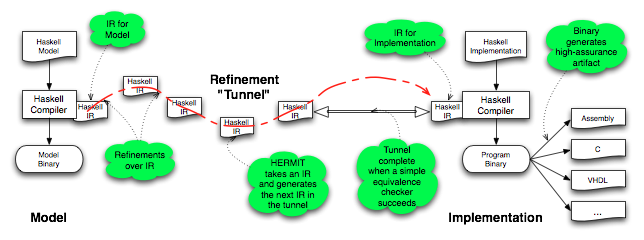
\includegraphics[width=0.235\textwidth]{html/HERMIT-tunnel.png}
\end{center}



\FurtherReading
  \url{http://www.ittc.ku.edu/csdl/fpg/Tools/HERMIT}
\end{hcarentry}
